% Created by tikzDevice version 0.8.1 on 2015-06-10 21:23:14
% !TEX encoding = UTF-8 Unicode
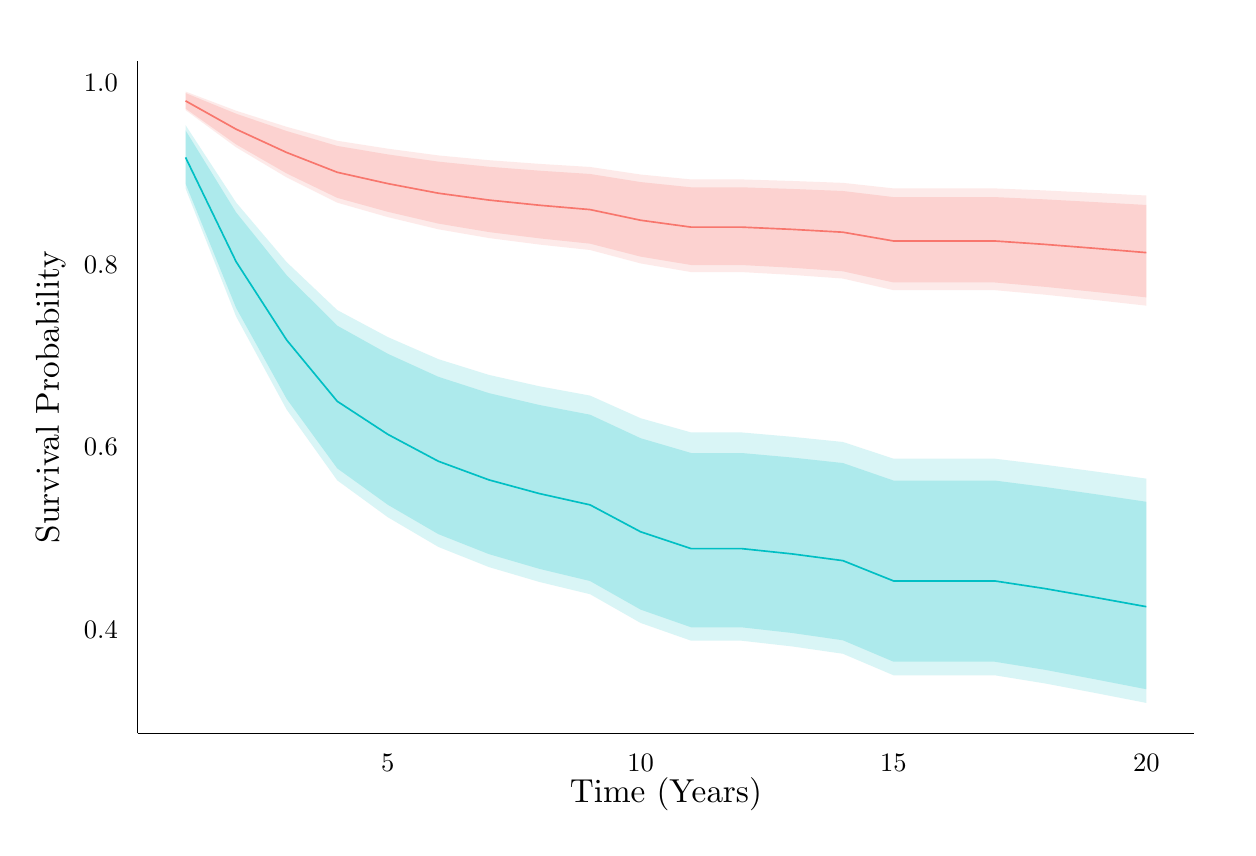
\begin{tikzpicture}[x=1pt,y=1pt]
\definecolor{fillColor}{RGB}{255,255,255}
\path[use as bounding box,fill=fillColor,fill opacity=0.00] (0,0) rectangle (433.62,289.08);
\begin{scope}
\path[clip] (  0.00,  0.00) rectangle (433.62,289.08);
\definecolor{drawColor}{RGB}{255,255,255}
\definecolor{fillColor}{RGB}{255,255,255}

\path[draw=drawColor,line width= 0.6pt,line join=round,line cap=round,fill=fillColor] (  0.00,  0.00) rectangle (433.62,289.08);
\end{scope}
\begin{scope}
\path[clip] ( 39.69, 34.03) rectangle (421.57,277.03);
\definecolor{fillColor}{RGB}{255,255,255}

\path[fill=fillColor] ( 39.69, 34.03) rectangle (421.58,277.03);
\definecolor{drawColor}{RGB}{248,118,109}

\path[draw=drawColor,line width= 0.6pt,line join=round] ( 57.05,262.62) --
	( 75.32,252.39) --
	( 93.59,243.97) --
	(111.86,236.82) --
	(130.13,232.73) --
	(148.41,229.26) --
	(166.68,226.78) --
	(184.95,224.91) --
	(203.22,223.34) --
	(221.49,219.49) --
	(239.77,217.00) --
	(258.04,217.00) --
	(276.31,216.19) --
	(294.58,215.17) --
	(312.86,212.00) --
	(331.13,212.00) --
	(349.40,212.00) --
	(367.67,210.76) --
	(385.94,209.32) --
	(404.22,207.79);
\definecolor{drawColor}{RGB}{0,191,196}

\path[draw=drawColor,line width= 0.6pt,line join=round] ( 57.05,242.19) --
	( 75.32,204.51) --
	( 93.59,176.21) --
	(111.86,154.07) --
	(130.13,142.13) --
	(148.41,132.40) --
	(166.68,125.67) --
	(184.95,120.71) --
	(203.22,116.64) --
	(221.49,106.91) --
	(239.77,100.83) --
	(258.04,100.83) --
	(276.31, 98.91) --
	(294.58, 96.49) --
	(312.86, 89.16) --
	(331.13, 89.16) --
	(349.40, 89.16) --
	(367.67, 86.38) --
	(385.94, 83.17) --
	(404.22, 79.85);
\definecolor{fillColor}{RGB}{248,118,109}

\path[fill=fillColor,fill opacity=0.15] ( 57.05,265.99) --
	( 75.32,259.07) --
	( 93.59,253.24) --
	(111.86,248.21) --
	(130.13,245.35) --
	(148.41,242.91) --
	(166.68,241.19) --
	(184.95,239.86) --
	(203.22,238.74) --
	(221.49,236.01) --
	(239.77,234.24) --
	(258.04,234.24) --
	(276.31,233.68) --
	(294.58,233.00) --
	(312.86,231.00) --
	(331.13,231.00) --
	(349.40,231.00) --
	(367.67,230.25) --
	(385.94,229.36) --
	(404.22,228.43) --
	(404.22,188.63) --
	(385.94,190.66) --
	(367.67,192.59) --
	(349.40,194.23) --
	(331.13,194.23) --
	(312.86,194.23) --
	(294.58,198.42) --
	(276.31,199.74) --
	(258.04,200.76) --
	(239.77,200.76) --
	(221.49,203.89) --
	(203.22,208.74) --
	(184.95,210.70) --
	(166.68,213.06) --
	(148.41,216.22) --
	(130.13,220.63) --
	(111.86,225.85) --
	( 93.59,234.97) --
	( 75.32,245.86) --
	( 57.05,259.28) --
	cycle;
\definecolor{fillColor}{RGB}{0,191,196}

\path[fill=fillColor,fill opacity=0.15] ( 57.05,253.85) --
	( 75.32,225.89) --
	( 93.59,204.35) --
	(111.86,187.03) --
	(130.13,177.28) --
	(148.41,169.30) --
	(166.68,163.60) --
	(184.95,159.49) --
	(203.22,156.13) --
	(221.49,147.95) --
	(239.77,142.81) --
	(258.04,142.81) --
	(276.31,141.23) --
	(294.58,139.37) --
	(312.86,133.34) --
	(331.13,133.34) --
	(349.40,133.34) --
	(367.67,131.12) --
	(385.94,128.68) --
	(404.22,126.12) --
	(404.22, 45.08) --
	(385.94, 48.64) --
	(367.67, 52.11) --
	(349.40, 55.07) --
	(331.13, 55.07) --
	(312.86, 55.07) --
	(294.58, 62.84) --
	(276.31, 65.48) --
	(258.04, 67.55) --
	(239.77, 67.55) --
	(221.49, 73.97) --
	(203.22, 84.36) --
	(184.95, 88.78) --
	(166.68, 94.16) --
	(148.41,101.44) --
	(130.13,112.18) --
	(111.86,125.50) --
	( 93.59,151.07) --
	( 75.32,184.72) --
	( 57.05,230.97) --
	cycle;
\definecolor{fillColor}{RGB}{248,118,109}

\path[fill=fillColor,fill opacity=0.20] ( 57.05,265.45) --
	( 75.32,257.99) --
	( 93.59,251.73) --
	(111.86,246.35) --
	(130.13,243.28) --
	(148.41,240.67) --
	(166.68,238.82) --
	(184.95,237.40) --
	(203.22,236.21) --
	(221.49,233.29) --
	(239.77,231.39) --
	(258.04,231.39) --
	(276.31,230.80) --
	(294.58,230.06) --
	(312.86,227.86) --
	(331.13,227.86) --
	(349.40,227.86) --
	(367.67,227.03) --
	(385.94,226.04) --
	(404.22,225.01) --
	(404.22,191.62) --
	(385.94,193.57) --
	(367.67,195.42) --
	(349.40,197.01) --
	(331.13,197.01) --
	(312.86,197.01) --
	(294.58,201.04) --
	(276.31,202.32) --
	(258.04,203.31) --
	(239.77,203.31) --
	(221.49,206.34) --
	(203.22,211.03) --
	(184.95,212.94) --
	(166.68,215.22) --
	(148.41,218.28) --
	(130.13,222.54) --
	(111.86,227.58) --
	( 93.59,236.40) --
	( 75.32,246.90) --
	( 57.05,259.82) --
	cycle;
\definecolor{fillColor}{RGB}{0,191,196}

\path[fill=fillColor,fill opacity=0.20] ( 57.05,251.95) --
	( 75.32,222.34) --
	( 93.59,199.61) --
	(111.86,181.41) --
	(130.13,171.24) --
	(148.41,162.92) --
	(166.68,157.02) --
	(184.95,152.73) --
	(203.22,149.23) --
	(221.49,140.73) --
	(239.77,135.38) --
	(258.04,135.38) --
	(276.31,133.74) --
	(294.58,131.76) --
	(312.86,125.44) --
	(331.13,125.44) --
	(349.40,125.44) --
	(367.67,123.10) --
	(385.94,120.49) --
	(404.22,117.76) --
	(404.22, 50.02) --
	(385.94, 53.57) --
	(367.67, 57.03) --
	(349.40, 59.97) --
	(331.13, 59.97) --
	(312.86, 59.97) --
	(294.58, 67.71) --
	(276.31, 70.34) --
	(258.04, 72.39) --
	(239.77, 72.39) --
	(221.49, 78.79) --
	(203.22, 89.12) --
	(184.95, 93.51) --
	(166.68, 98.84) --
	(148.41,106.06) --
	(130.13,116.68) --
	(111.86,129.83) --
	( 93.59,154.93) --
	( 75.32,187.80) --
	( 57.05,232.75) --
	cycle;
\end{scope}
\begin{scope}
\path[clip] (  0.00,  0.00) rectangle (433.62,289.08);
\definecolor{drawColor}{RGB}{0,0,0}

\path[draw=drawColor,line width= 0.6pt,line join=round] ( 39.69, 34.03) --
	( 39.69,277.03);
\end{scope}
\begin{scope}
\path[clip] (  0.00,  0.00) rectangle (433.62,289.08);
\definecolor{drawColor}{RGB}{0,0,0}

\node[text=drawColor,anchor=base east,inner sep=0pt, outer sep=0pt, scale=  0.96] at ( 32.57, 68.41) {0.4};

\node[text=drawColor,anchor=base east,inner sep=0pt, outer sep=0pt, scale=  0.96] at ( 32.57,134.31) {0.6};

\node[text=drawColor,anchor=base east,inner sep=0pt, outer sep=0pt, scale=  0.96] at ( 32.57,200.21) {0.8};

\node[text=drawColor,anchor=base east,inner sep=0pt, outer sep=0pt, scale=  0.96] at ( 32.57,266.11) {1.0};
\end{scope}
\begin{scope}
\path[clip] (  0.00,  0.00) rectangle (433.62,289.08);
\definecolor{drawColor}{RGB}{0,0,0}

\path[draw=drawColor,line width= 0.6pt,line join=round] ( 39.69, 34.03) --
	(421.57, 34.03);
\end{scope}
\begin{scope}
\path[clip] (  0.00,  0.00) rectangle (433.62,289.08);
\definecolor{drawColor}{RGB}{0,0,0}

\node[text=drawColor,anchor=base,inner sep=0pt, outer sep=0pt, scale=  0.96] at (130.13, 20.31) {5};

\node[text=drawColor,anchor=base,inner sep=0pt, outer sep=0pt, scale=  0.96] at (221.49, 20.31) {10};

\node[text=drawColor,anchor=base,inner sep=0pt, outer sep=0pt, scale=  0.96] at (312.86, 20.31) {15};

\node[text=drawColor,anchor=base,inner sep=0pt, outer sep=0pt, scale=  0.96] at (404.22, 20.31) {20};
\end{scope}
\begin{scope}
\path[clip] (  0.00,  0.00) rectangle (433.62,289.08);
\definecolor{drawColor}{RGB}{0,0,0}

\node[text=drawColor,anchor=base,inner sep=0pt, outer sep=0pt, scale=  1.20] at (230.63,  9.03) {Time (Years)};
\end{scope}
\begin{scope}
\path[clip] (  0.00,  0.00) rectangle (433.62,289.08);
\definecolor{drawColor}{RGB}{0,0,0}

\node[text=drawColor,rotate= 90.00,anchor=base,inner sep=0pt, outer sep=0pt, scale=  1.20] at ( 11.28,155.53) {Survival Probability};
\end{scope}
\end{tikzpicture}
